%! TeX program = lualatex
\documentclass[../main.tex]{subfiles}
\begin{document} \section{Linear vector fields}\label{sec:linalg-vector-fields}

A vector field is a way to visualize \hlattn{changes} in a system. Let's see the idea through examples. A \hlmain{linear vector field} is a vector field to describe \hlattn{change} encoded by the recurrence equation \(\vec{x}(t+1) = A \vec{x}(t)\).  We will see non-linear vector fields for the famous Lokta-Volterra equations in about two to three weeks.

\begin{example} \label{ex:linear-vector-field-intro}
  Let \(A = \begin{bmatrix} 0 & 0.1 \\ 0.2 & 0.8 \end{bmatrix}\) and \(\vec{x}(0) = \begin{bmatrix} 30 \\ 20 \end{bmatrix}\).
  Calculate and plot \(\vec{x}(0), \vec{x}(1), \vec{x}(2), \vec{x}(3)\).

  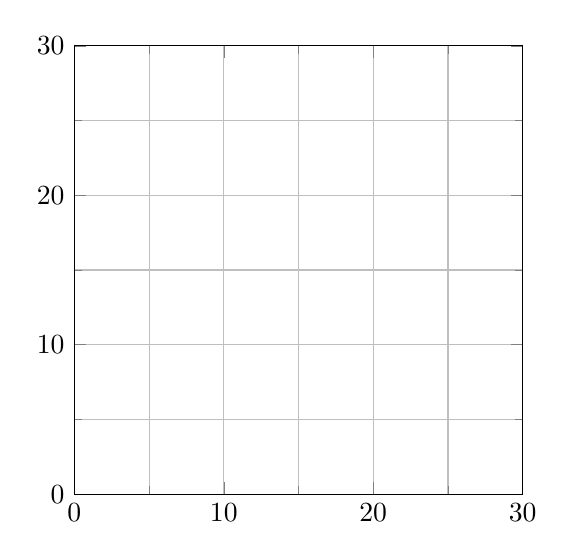
\begin{tikzpicture}[scale=1]
    \begin{axis}[xmin=0, xmax=30, ymin=0, ymax=30, minor tick num=1, grid=both, axis equal image]
    \end{axis}
  \end{tikzpicture}
\end{example}

To create the vector field for recurrence equations \(\vec{x}(t+1) = A \vec{x}(t)\), we plot arrows starting at \(\vec{v}\) ending at \(A \vec{v}\) for enough \(\vec{v}\). Clearly, plotting linear vector fields is a job for the computer. 

However, we should understand that \emph{linear vector fields} are really just a fancy term for ``\emph{\hlattn{change} matricies}'' which will come up again when we discuss systems of differential equations.

\blanklines{20}

\clearpage
Vectors fields visualize motion encoded by recurrence equations \(\vec{x}(t+1) = A \vec{x}(t)\).  If we were to visually solve such a recurrence, we simply follow the arrows starting at some initial condition \(\vec{x}(0)\).

\begin{example}
  The following are vector fields for two systems of recurrence equations.  Use the vector field to find the long-term behaviour for a recurrence with initial condition \(\vec{x}(0) = \begin{bmatrix} -50 \\ -50 \end{bmatrix}\).

  \begin{center}
    \includegraphics{../standalones/build/plot_vector_field_rotation2}
    \quad
    \includegraphics{../standalones/build/plot_vector_field_rotation3}
  \end{center}
\end{example}
\vfill{}

Sometimes, we scale the arrows in a vector field so that the plot is more readable. 
\begin{example}
  Here are the vector fields for the system of recurrence equations in Example~\ref{ex:linear-vector-field-intro}. The one on the left is not scaled. The one on the right is scaled.

  Sketch the long-term behaviour for a recurrence with initial condition \(\vec{x}(0) = \begin{bmatrix} 30 \\ 20 \end{bmatrix}\).  Does the sketch match the calculations in Example~\ref{ex:linear-vector-field-intro}?


  \begin{center}
    \includegraphics{../standalones/build/plot_vector_field_intro}
    \quad
    \includegraphics{../standalones/build/plot_vector_field_intro_scaled}
  \end{center}
\end{example}
\vfill{}
\clearpage

\begin{example}
  The two vector field plots below come from the same recurrence equations. The one on the left is not scaled. The one on the right is scaled. 

  Use both vector field below to sketch the long-term behaviour for a recurrence with initial condition \(\vec{x}(0) = \begin{bmatrix} 80 \\ 0 \end{bmatrix}\). Are the results really different?

  \begin{center}
    \includegraphics{../standalones/build/plot_vector_field_rotation}
    \quad
    \includegraphics{../standalones/build/plot_vector_field_rotation_scaled}
  \end{center}
\end{example}

\end{document}
